\section{Resultados}

En esta sección, se comentarán los resultados obtenidos tras la investigación realizada. Dicha investigación ha tomado los siguientes pasos: búsqueda de proteínas virales del SARS-CoV2 y genes asociados a ellas, búsqueda de las enfermedades relacionadas con los genes de las proteínas y desarrollo de código para el análisis de red PPI.

\newline

Para la primera parte de la ejecución se cargaron los datos recopilados en \textit{STRING}, es decir, los genes asociados a las proteínas virales del virus. Tras agrupar todos los datos, se creó un objeto de \textit{STRINGdb}, se mapeó y se generó la red de interacción. A continuación, podemos observar la siguiente red obtenida.

\newline

\begin{figure}[h!]
	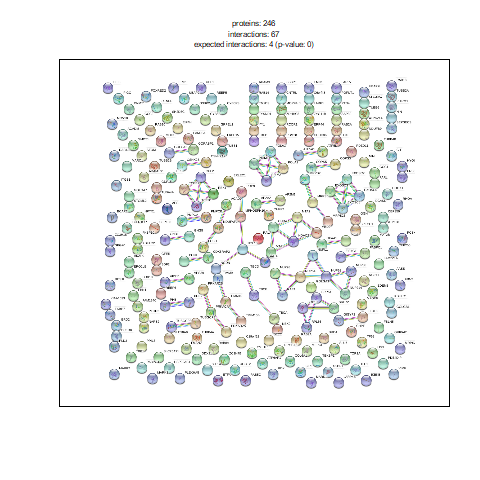
\includegraphics[width=0.9\textwidth]{../../results/figuraSTRINGdb.png}
	\caption{Interacciones entre genes obtenida por medio de STRINGdb}
	\label{fig:red_stringdb}
\end{figure}

\newline

En dicha figura se muestra una representación de los genes recopilados interaccionando entre ellos pero en la especie \textit{Homo Sapiens}. Se puede observar que en esta especie hay 67 interacciones entre los 246 genes considerados, por lo cual existen bastantes genes que no interaccionan entre ellos.

\newline

Para la segunda parte de la ejecución del código era necesario realizar la búsqueda de enfermedades asociadas a los diferentes genes por medio de \textit{PheGenI} y guardar estas relaciones en una determinada variable para su uso. Se obtuvo 75 genes con enfermedades asociadas, y para este conjunto se ploteó una red de interacción entre genes y enfermedades por medio de \textit{igraph}. La red obtenida se muestra a continuación.

\newline

\begin{figure}[h!]
	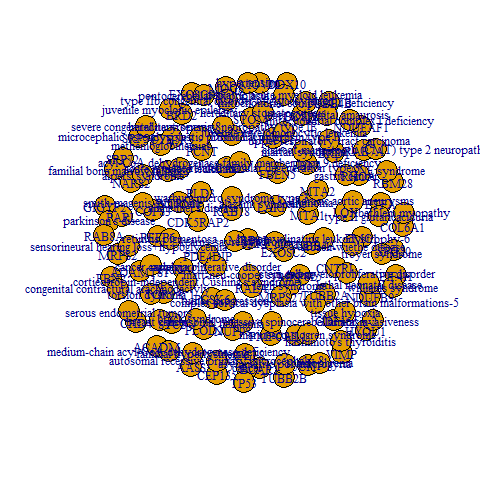
\includegraphics[width=0.9\textwidth]{../../results/figuraiGraph.png}
	\caption{Interacciones genes y enfermedades obtenida por medio de igraph}
	\label{fig:red_igraph}
\end{figure}

\newline

Debido a que no se observaba una clara diferencia entre los nodos, se decidió hacer uso de la librería \textit{linkcomm}.

\newline

Para la tercera y última parte de la ejecución, se generó una red de interacción entre genes y enfermedades en la que se mostrase las comunidades existentes en dicha red. La red creada corresponde con la mostrada a continuación.

\newline

\begin{figure}[h!]
	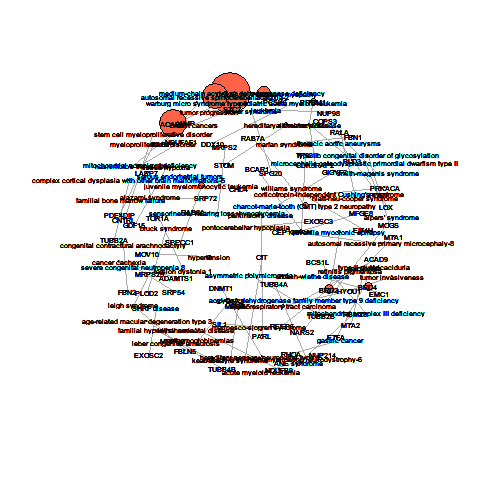
\includegraphics[width=0.9\textwidth]{../../results/figuraLinkcomm.png}
	\caption{Interacciones genes y enfermedades obtenida por medio de LinkComm}
	\label{fig:red_linkcomm}
\end{figure}

\newline

Se puede observar que gran parte de las enfermedades están asociadas a un solo gen, pero existen algunas que tienen varios genes asociados. 

\newline

Durante la búsqueda de enfermedades relacionadas, se pudo observar que enfermedades como el cáncer, la enfermedad de Parkinson, el Alzheimer o el carcinoma, están relacionadas con varios genes. Esto quiere decir que el individuo con dichas enfermedades será más susceptible a contagiase por COVID-19. Por otro lado, con el resto de enfermedades asociadas ocurrirá lo mismo, aunque las nombradas previamente están asociadas a más de las proteínas estudiadas en esta investigación.

\newline

A modo de interés, las enfermedades que se obtuvieron tras la búsqueda y que por lo tanto, están relacionadas con la susceptibilidad de contraer la enfermedad COVID-19, son \textit{juvenile myoclonic epilepsy, upper respiratory tract carcinoma, familial hyperlysinemia, medium-chain acyl-CoA dehydrogenase deficiency, type II glutaricaciduria, alzheimer's disease, autosomal recessive spinocerebellar ataxia-2, retinitis pigmentosa, hereditary stomatocytosis, hypertension, ANE syndrome, parkinson's disease, cancer, juvenile myelomonocytic leukemia, serous endometrial tumors, hereditary sensory neuropathy type IE, carcinoma, methemoglobinemias, type IIb congenital disorder of glycosylation, warburg micro syndrome type 3, charcot-marie-tooth (CMT) type 2 neuropathy, hiatt-neu-cooper syndrome, gastric cancer, hashimoto's thyroiditis, pediatric acute myeloid leukemia, SHRF disease, pontocerebellar hypoplasia, alazami syndrome, sensorineural hearing loss+hypoglycemia, leigh syndrome, kearns-sayre syndrome, alpers' syndrome, severe congenital neutropenia 8, familial bone marrow failure, williams syndrome, age-related macular degeneration type 3, marfan syndrome, congenital contractural arachnodactyly, acute myeloid leukemia, troyer syndrome, complex cortical dysplasia with other brain malformations-5, asymmetric polymicrogyria, hypomyelinating leukodystrophy-6, leber congenital amaurosis, autosomal recessive primary microcephaly-8, schizophrenia, stem cell myeloproliferative disorder, microcephalic osteodysplastic primordial,  dwarfism type II, myeloproliferative disorder, corticotropin-independent Cushing's syndrome, smith-magenis syndrome, leukemia, cancer cachexia, bethlem myopathy, urbach-wiethe disease, tissue hypoxia, tumor invasiveness, thoracic aortic aneurysms, tumor progression, bruck syndrome, marinesco-sjogren syndrome, breast cancers, torsion dystonia 1, acyl-CoA dehydrogenase family member type 9 deficiency, mitochondrial complex III deficiency, mitochondrial complex I deficiency, lethal neonatal disease}.